\chapter{Анализ разработанной системы}

В результате разработки была реализована возможность интеграции  аналитических отчётов платформы бизнес-аналитики в CRM-систему Vtiger.

Интеграция происходит с помощью веб-сервиса, находящегося на сервере Pentaho. С помощью приложения возможно передать данные из отчёта OLAP-аналитики с сервера Pentaho CRM-системе.

По итогам исследования было выяснено, что инструменты аналитики CRM Vtiger недостаточно мощны для комплексного анализа. Реализованное приложение даёт возможность предоставить результаты работы OLAP-анализатора Saiku платформы Pentaho BI по REST-протоколу.

Продемонстрируем работу созданного приложения. У нас уже имеется аналитический отчёт, созданный в Saiku и открытый рассматриваемым плагином. Отсёт продемонстрирован на рисунке \ref{fig:table} С этого момента уже возможно получить доступ к данным в отчёте, введя URL-адрес REST-сервиса с корректными параметрами. 

\begin{figure}[htbp]
	\centering
	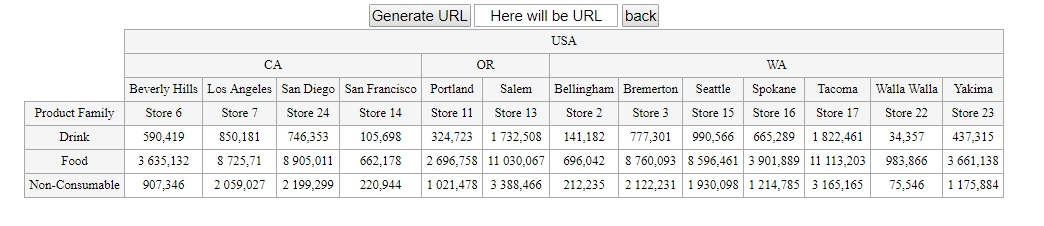
\includegraphics[width=0.9\textwidth]{fig/chapter_6/table}
	\caption{Отчёт в разработанном плагине}
	\label{fig:table}
\end{figure}

Выберем данные для генерации URL-адреса и сгенерируем его, нажав на соответствующую кнопку в интерфейсе. Результат демонстрирует рисунок \ref{fig:gen_url1}.

\begin{figure}[htbp]
	\centering
	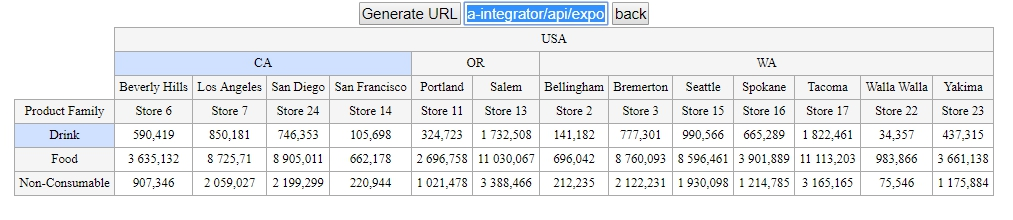
\includegraphics[width=0.9\textwidth]{fig/chapter_6/gen_url1}
	\caption{Выбор данных для генерации URL}
	\label{fig:gen_url1}
\end{figure}

Далее можно использовать данный URL для дальнейшего использования результатов работы аналитического отчёта. Для этого создадим страницу с параграфом, что поместить туда полученный json-объект. Пример показан на рисунке \ref{fig:gen_url2}

\begin{figure}[htbp]
	\centering
	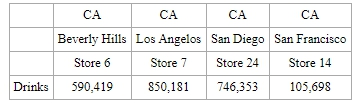
\includegraphics[width=0.6\textwidth]{fig/chapter_6/gen_url2}
	\caption{Демонстрация REST-сервиса}
	\label{fig:gen_url2}
\end{figure}

Таким образом, можно сказать, что задача выполнена. С помощью разработанного плагина можно посредством REST-протокола предоставлять доступ к ресурсам отчётов системы Pentaho BI Suite.